\section*{Appendice}
\addcontentsline{toc}{section}{Appendice}

\begin{figure}[H]
    \centering
    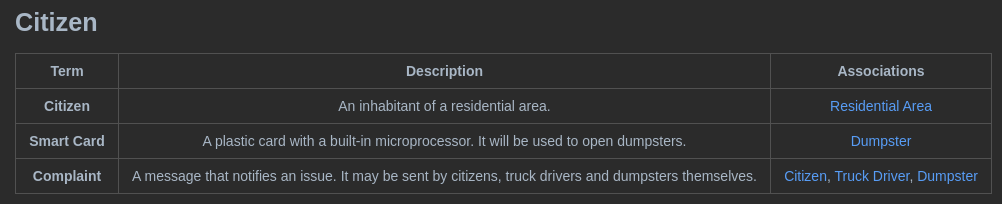
\includegraphics[width=\textwidth]{img/citizen-ubiquitous-language}
    \caption{\textit{Ubiquitous Language}: i termini del topic "cittadino". \hyperlink{back:img/citizen-ubiquitous-language}{Torna indietro}.}
    \label{fig:img/citizen-ubiquitous-language}
\end{figure}


\begin{figure}[H]
    \centering
    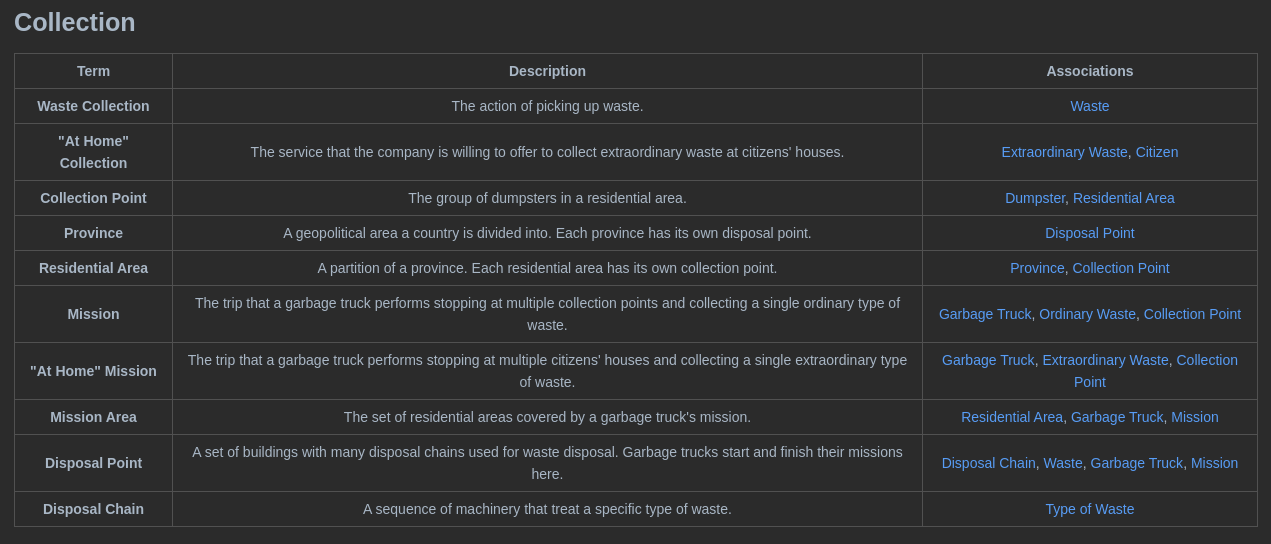
\includegraphics[width=\textwidth]{img/collection-ubiquitous-language}
    \caption{\textit{Ubiquitous Language}: i termini del topic "raccolta". \hyperlink{back:img/collection-ubiquitous-language}{Torna indietro}.}
    \label{fig:img/collection-ubiquitous-language}
\end{figure}


\begin{figure}[H]
    \centering
    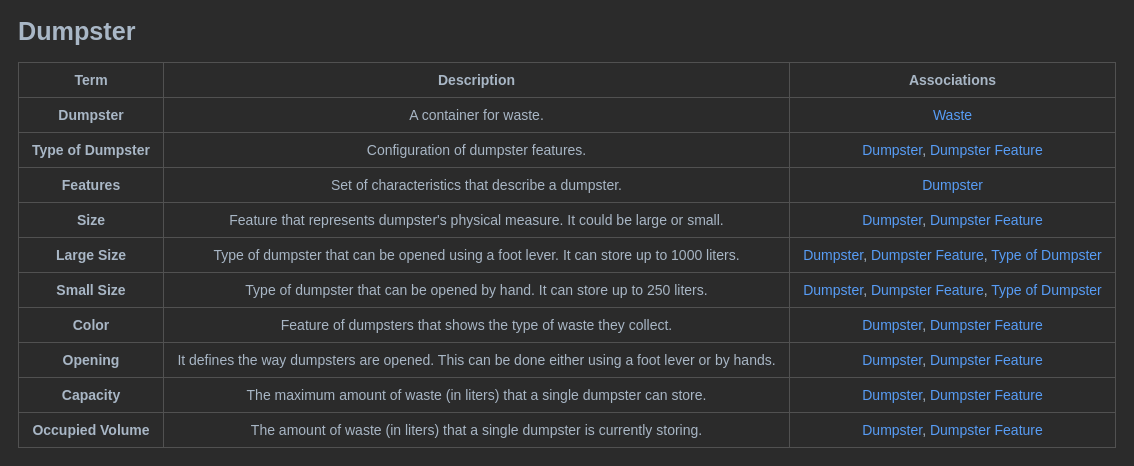
\includegraphics[width=\textwidth]{img/dumpster-ubiquitous-language}
    \caption{\textit{Ubiquitous Language}: i termini del topic "cassonetti". \hyperlink{back:img/dumpster-ubiquitous-language}{Torna indietro}.}
    \label{fig:img/dumpster-ubiquitous-language}
\end{figure}


\begin{figure}[H]
    \centering
    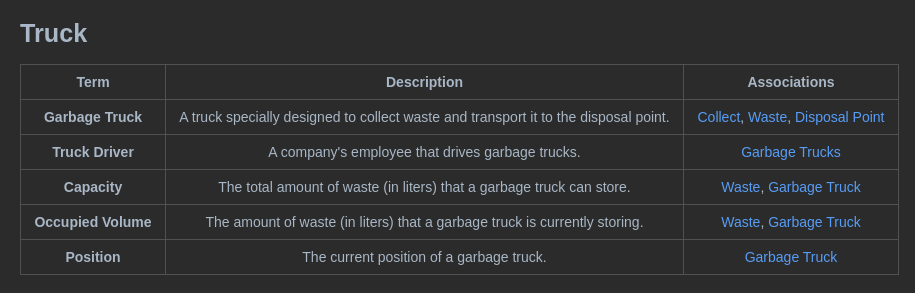
\includegraphics[width=\textwidth]{img/truck-ubiquitous-language}
    \caption{\textit{Ubiquitous Language}: i termini del topic "camioncini". \hyperlink{back:img/truck-ubiquitous-language}{Torna indietro}.}
    \label{fig:img/truck-ubiquitous-language}
\end{figure}


\begin{figure}[H]
    \centering
    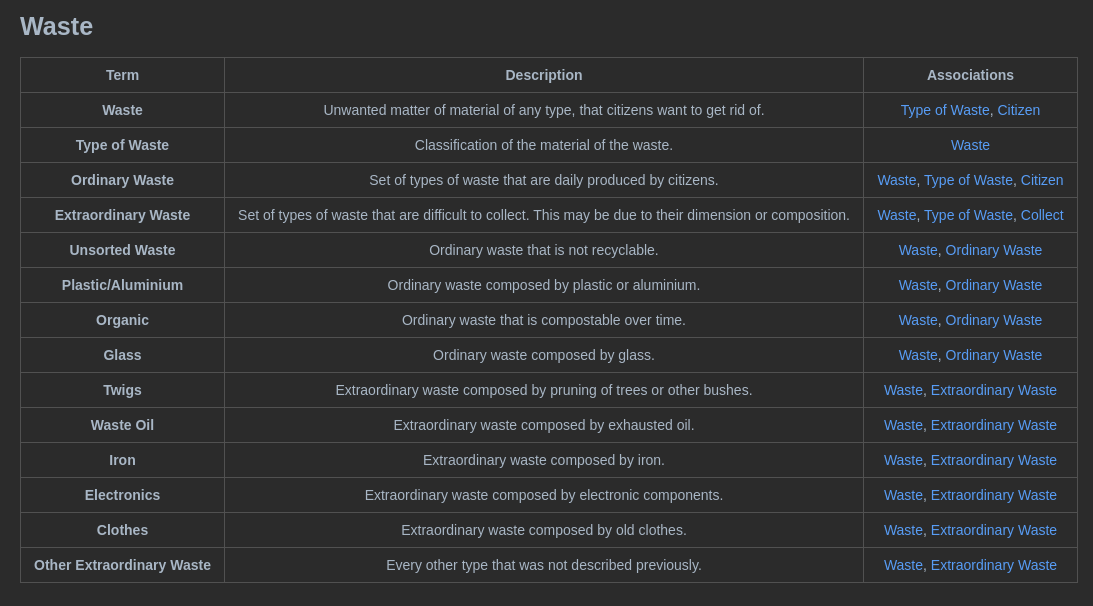
\includegraphics[width=\textwidth]{img/waste-ubiquitous-language}
    \caption{\textit{Ubiquitous Language}: i termini del topic "rifiuti". \hyperlink{back:img/waste-ubiquitous-language}{Torna indietro}.}
    \label{fig:img/waste-ubiquitous-language}
\end{figure}


\begin{figure}[H]
    \centering
    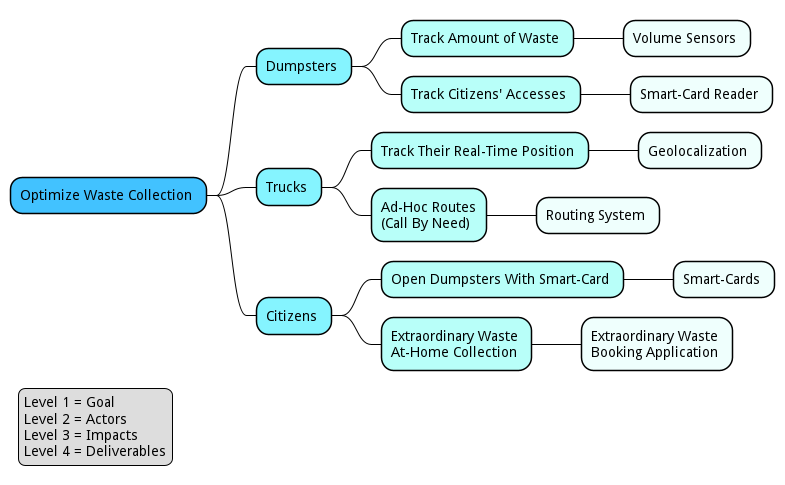
\includegraphics[width=\textwidth]{uml/impact-mapping.pm}
    \caption{\textit{Impact map} che, a partire dal \textit{goal}, mostra quali sono le soluzioni con maggiore impatto sugli attori del sistema. \hyperlink{back:uml/impact-mapping}{Torna indietro}.}
    \label{fig:uml/impact-mapping}
\end{figure}


\begin{figure}[H]
    \centering
    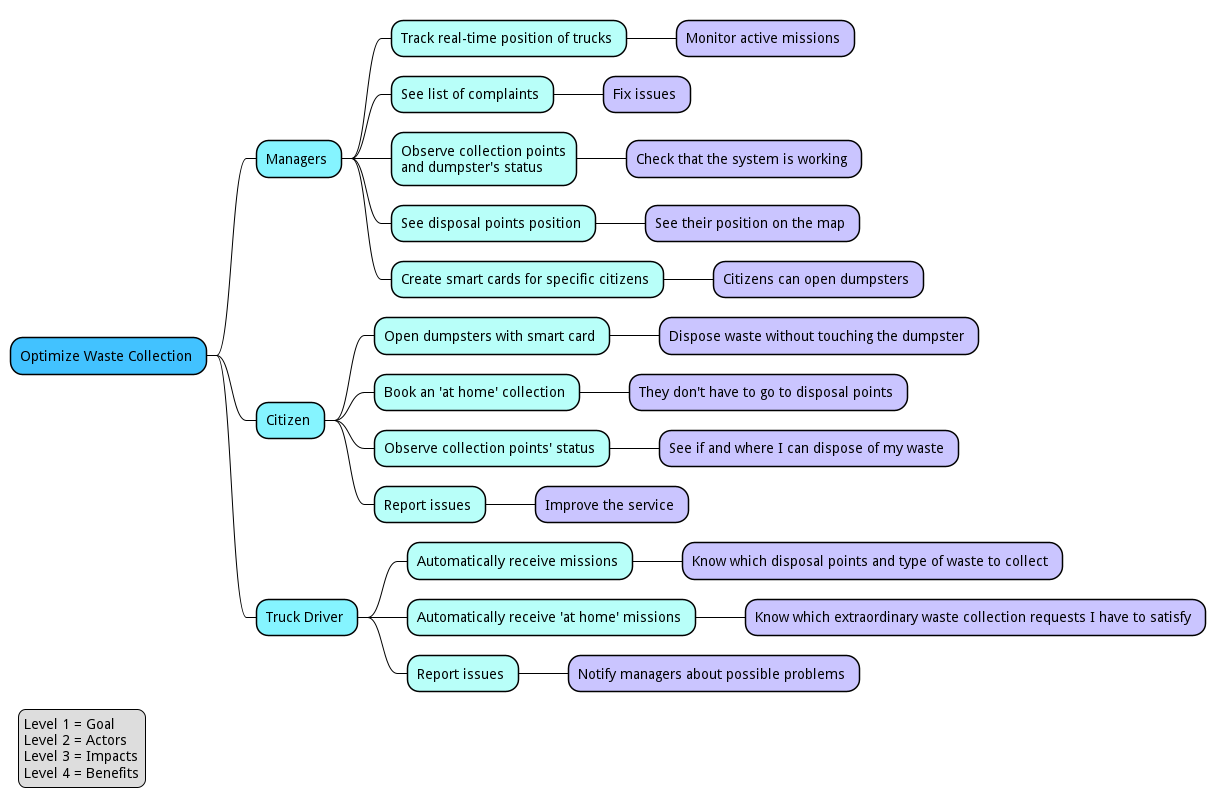
\includegraphics[width=\textwidth]{uml/benefit-mapping.pm}
    \caption{\textit{Impact map} che, a partire dal \textit{goal}, mostra chi sono gli attori che beneficiano maggiormente dai cambiamenti introdotti dal sistema. \hyperlink{back:uml/benefit-mapping}{Torna indietro}.}
    \label{fig:uml/benefit-mapping}
\end{figure}


\begin{figure}[H]
    \centering
    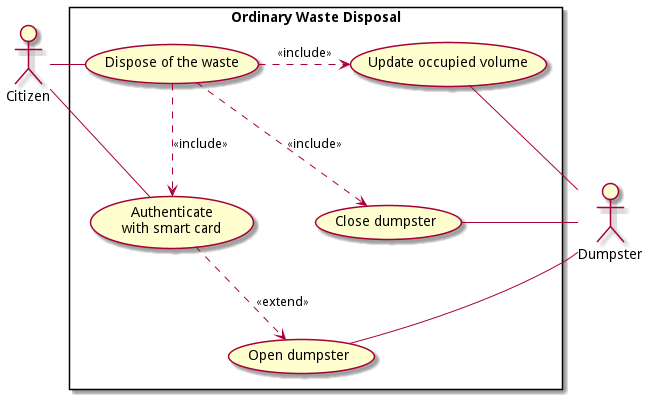
\includegraphics[width=\textwidth]{uml/ordinary-disposal-use-cases.pm}
    \caption{Diagramma dei casi d'uso dello scenario del conferimento di rifiuti ordinari. \hyperlink{back:uml/ordinary-disposal-use-cases}{Torna indietro}.}
    \label{fig:uml/ordinary-disposal-use-cases}
\end{figure}


\begin{figure}[H]
    \centering
    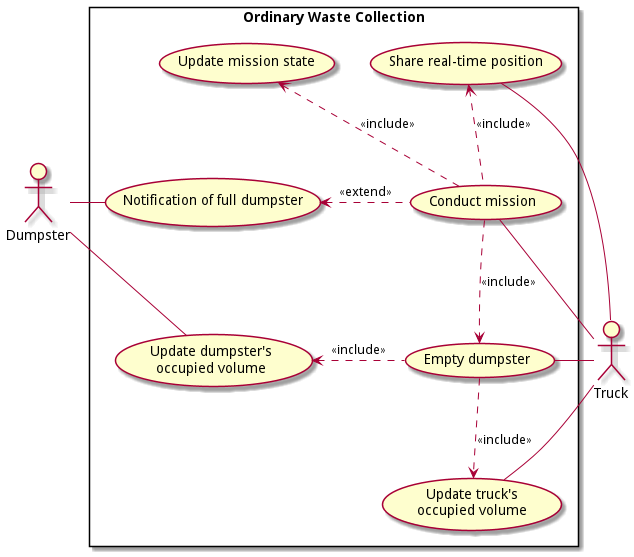
\includegraphics[width=\textwidth]{uml/ordinary-collection-use-cases.pm}
    \caption{Diagramma dei casi d'uso dello scenario della raccolta di rifiuti ordinari. \hyperlink{back:uml/ordinary-collection-use-cases}{Torna indietro}.}
    \label{fig:uml/ordinary-collection-use-cases}
\end{figure}


\begin{figure}[H]
    \centering
    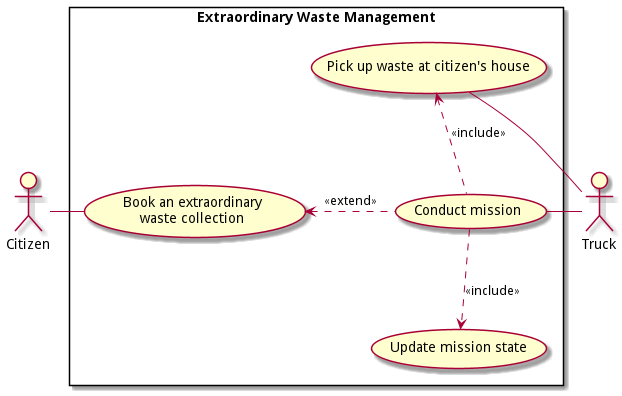
\includegraphics[width=\textwidth]{uml/extraordinary-management-use-cases.pm}
    \caption{Diagramma dei casi d'uso dello scenario della gestione di rifiuti straordinari. \hyperlink{back:uml/extraordinary-management-use-cases}{Torna indietro}.}
    \label{fig:uml/extraordinary-management-use-cases}
\end{figure}


\begin{figure}[H]
    \centering
    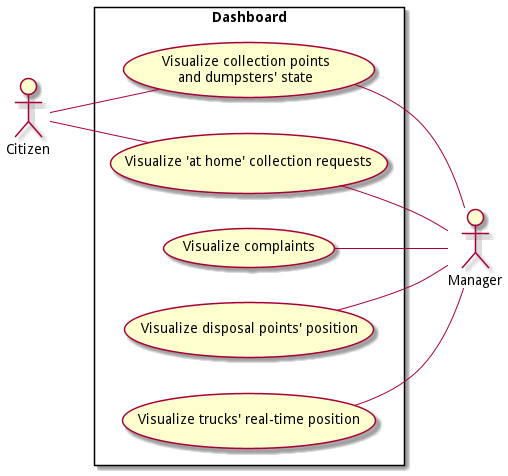
\includegraphics[width=\textwidth]{uml/dashboard-use-cases.pm}
    \caption{Diagramma dei casi d'uso dello scenario dell'utilizzo della dashboard. \hyperlink{back:uml/dashboard-use-cases}{Torna indietro}.}
    \label{fig:uml/dashboard-use-cases}
\end{figure}


\begin{figure}[H]
    \centering
    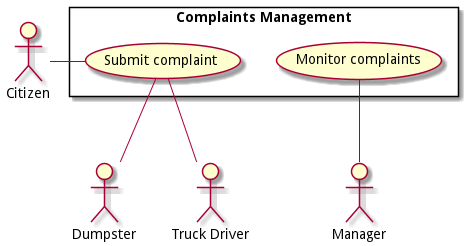
\includegraphics[width=\textwidth]{uml/complaints-use-cases.pm}
    \caption{Diagramma dei casi d'uso dello scenario della gestione dei reclami. \hyperlink{back:uml/complaints-use-cases}{Torna indietro}.}
    \label{fig:uml/complaints-use-cases}
\end{figure}


\begin{figure}[H]
    \centering
    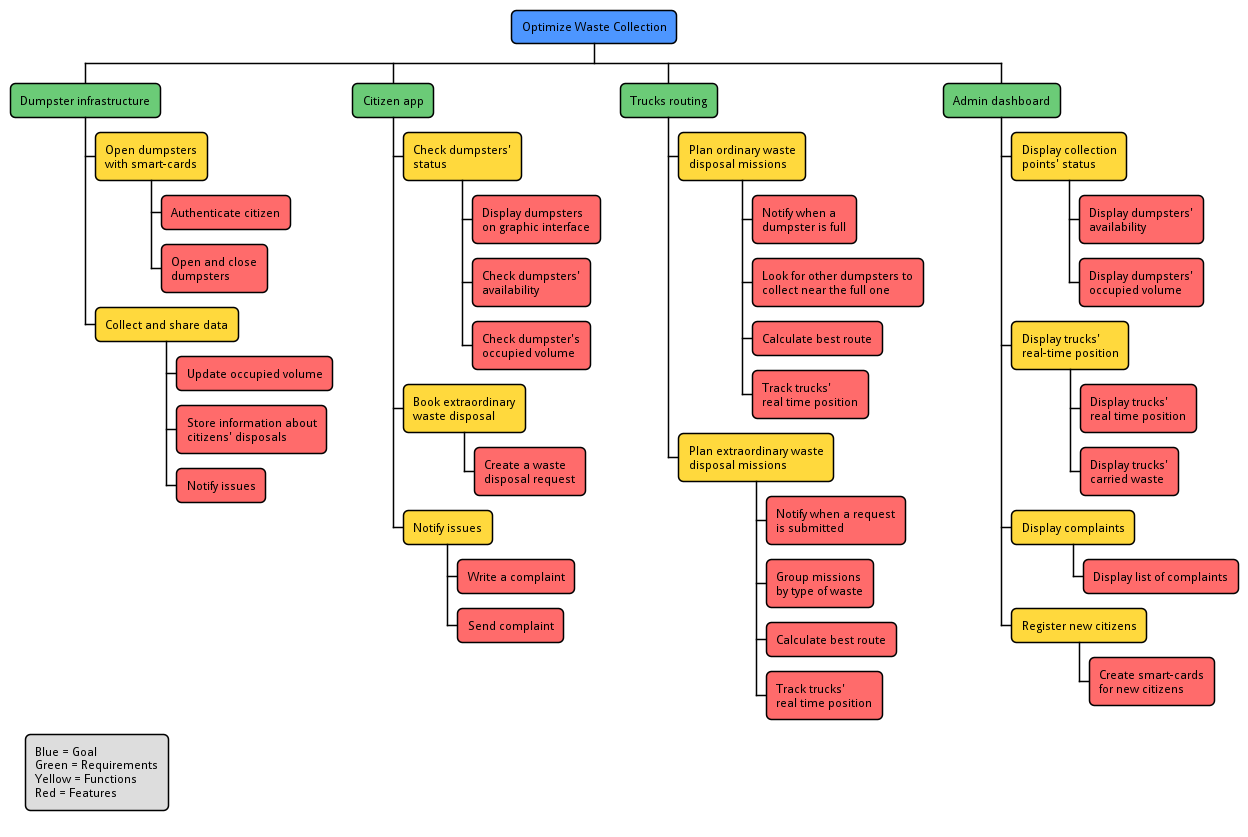
\includegraphics[width=\textwidth]{uml/requirement-breakdown-structure.pm}
    \caption{\textit{Requirement Breakdown Structure} derivata dall'analisi delle \textit{user stories} e parzialmente inclusa nel \textit{Project Overview Statement}   \hyperlink{back:uml/requirement-breakdown-structure}{Torna indietro}.}
    \label{fig:uml/requirement-breakdown-structure}
\end{figure}


\begin{figure}[H]
    \centering
    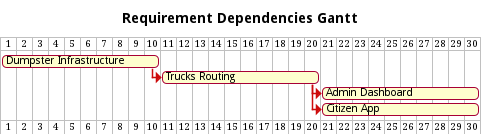
\includegraphics[width=\textwidth]{uml/gantt-requirements-dependencies.pm}
    \caption{ \hyperlink{back:uml/gantt-requirements-dependencies}{Torna indietro}.}
    \label{fig:uml/gantt-requirements-dependencies}
\end{figure}


\begin{figure}[H]
    \centering
    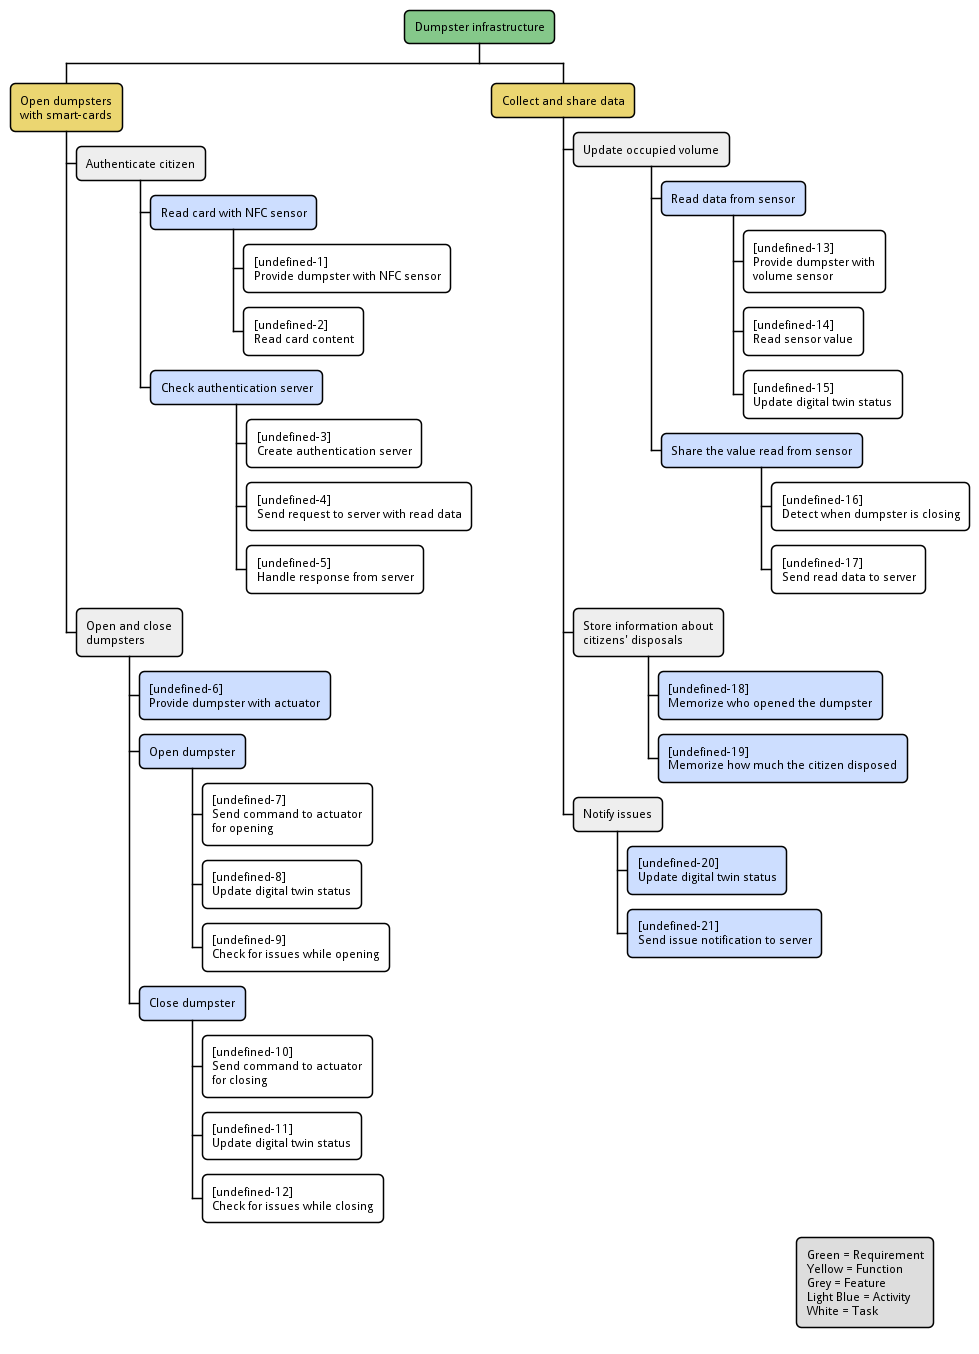
\includegraphics[width=\textwidth]{uml/wbs-dumpster-infrastructure.pm}
    \caption{\textit{Work Breakdown Structure} della \textbf{Dumpster Infrastructure}. \hyperlink{back:uml/wbs-dumpster-infrastructure}{Torna indietro}.}
    \label{fig:uml/wbs-dumpster-infrastructure}
\end{figure}


\begin{figure}[H]
    \centering
    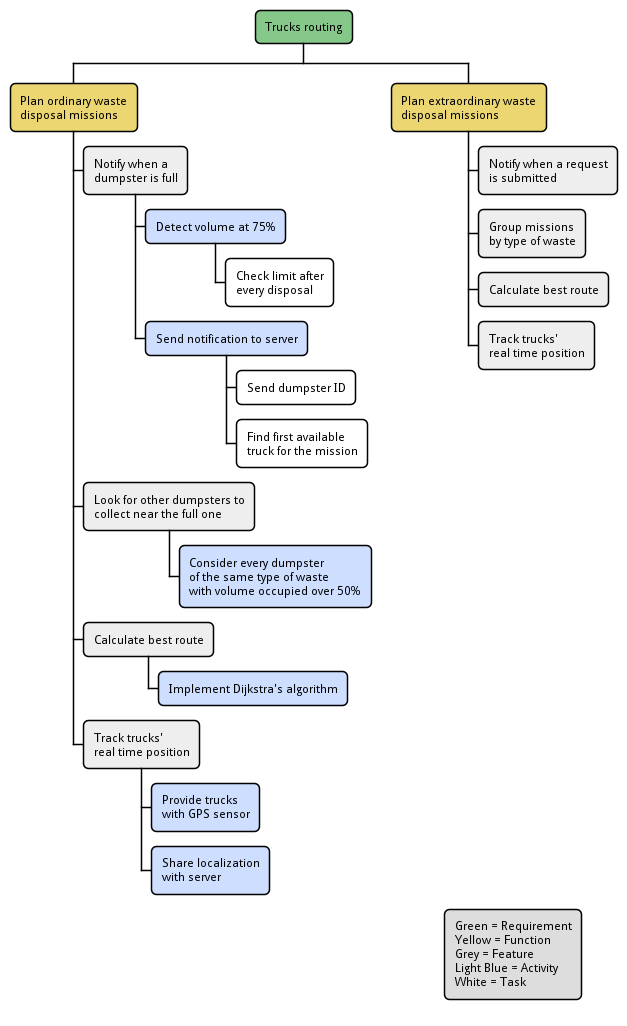
\includegraphics[width=\textwidth]{uml/wbs-trucks-routing.pm}
    \caption{\textit{Work Breakdown Structure} del \textbf{Trucks Routing}. \hyperlink{back:uml/wbs-trucks-routing}{Torna indietro}.}
    \label{fig:uml/wbs-trucks-routing}
\end{figure}


\begin{figure}[H]
    \centering
    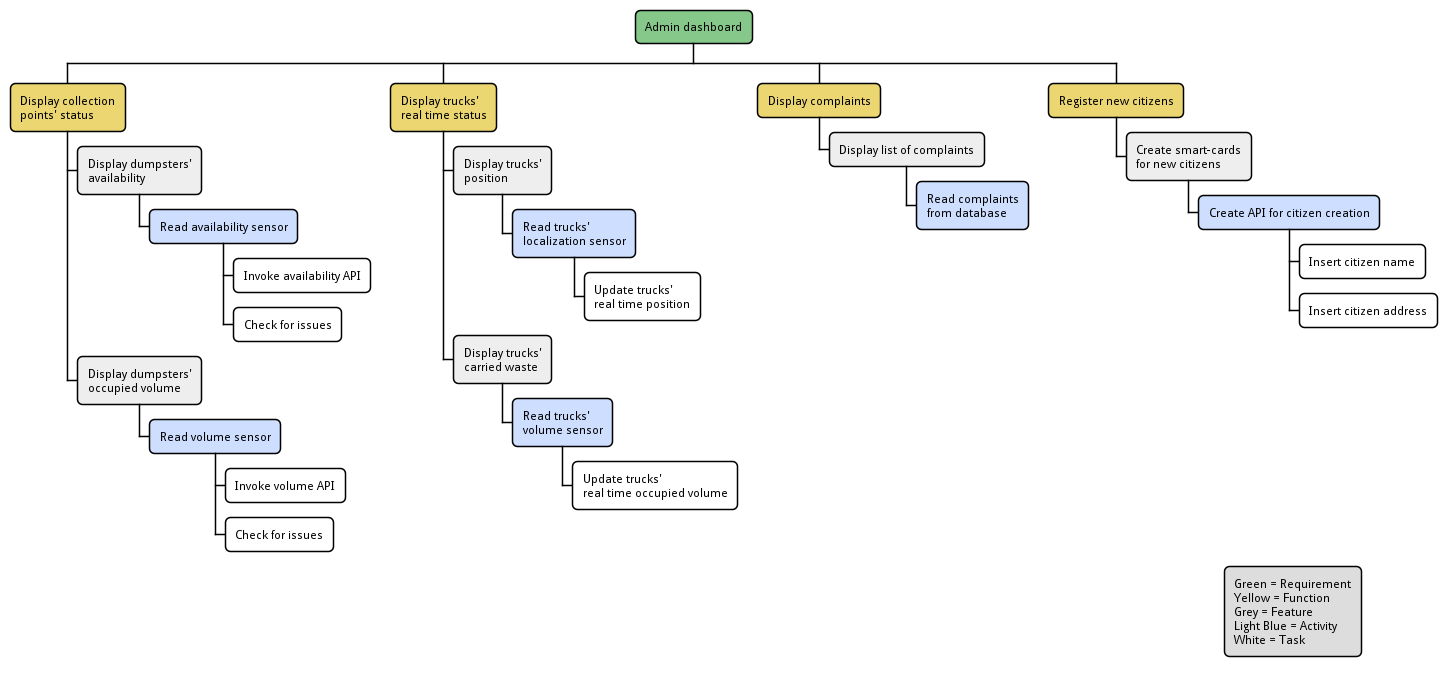
\includegraphics[width=\textwidth]{uml/wbs-admin-dashboard.pm}
    \caption{\textit{Work Breakdown Structure} della \textbf{Admin Dashboard}. \hyperlink{back:uml/wbs-admin-dashboard}{Torna indietro}.}
    \label{fig:uml/wbs-admin-dashboard}
\end{figure}


\begin{figure}[H]
    \centering
    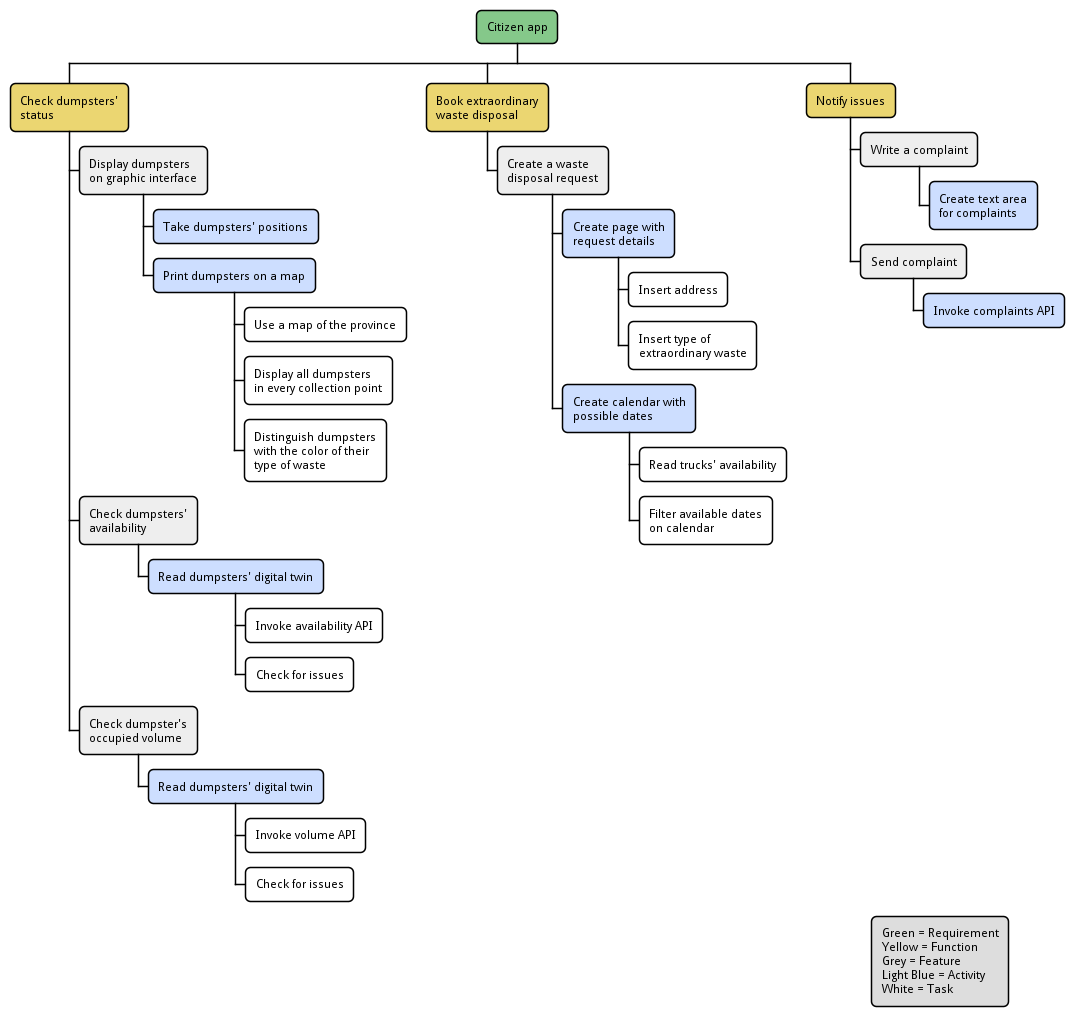
\includegraphics[width=\textwidth]{uml/wbs-citizen-app.pm}
    \caption{\textit{Work Breakdown Structure} della \textbf{Citizen App}. \hyperlink{back:uml/wbs-citizen-app}{Torna indietro}.}
    \label{fig:uml/wbs-citizen-app}
\end{figure}


\begin{figure}[H]
    \centering
    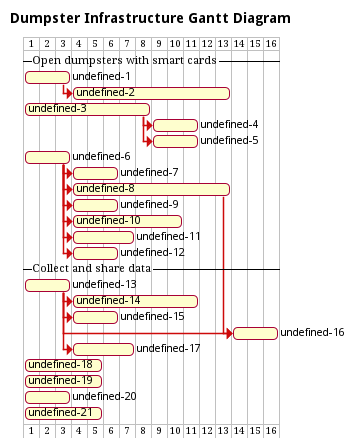
\includegraphics[width=\textwidth]{uml/gantt-dumpster-infrastructure.pm}
    \caption{Diagramma Gantt contenente le attività e i task per portare a termine la \textit{Dumpster Infrastructure}. \hyperlink{back:uml/gantt-dumpster-infrastructure}{Torna indietro}.}
    \label{fig:uml/gantt-dumpster-infrastructure}
\end{figure}


\begin{figure}[H]
    \centering
    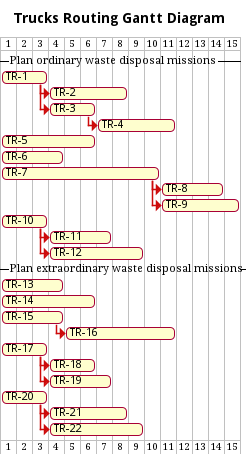
\includegraphics[width=\textwidth]{uml/gantt-trucks-routing.pm}
    \caption{Diagramma Gantt contenente le attività e i task per portare a termine il \textit{Trucks Routing}. \hyperlink{back:uml/gantt-trucks-routing}{Torna indietro}.}
    \label{fig:uml/gantt-trucks-routing}
\end{figure}


\begin{figure}[H]
    \centering
    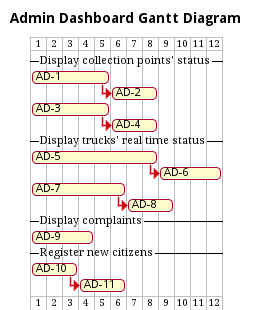
\includegraphics[width=\textwidth]{uml/gantt-admin-dashboard.pm}
    \caption{Diagramma Gantt contenente le attività e i task per portare a termine la \textit{Admin Dashboard}. \hyperlink{back:uml/gantt-admin-dashboard}{Torna indietro}.}
    \label{fig:uml/gantt-admin-dashboard}
\end{figure}

